\chapter{Additional \rmfamily{\LaTeX{}} Formatting}
\label{ch:ch2}

In this chapter, we'll provide some additional guidelines and useful \LaTeX{} commands for formatting your document.


%{\color{mediumgray} \blindtext}
\section{More {\rmfamily\LaTeX{}} Usage Examples}
In the \cref{fig:brach} below, we show some pretty blue and grey lines. This second figure in the document and the first in Chapter~\ref{ch:ch2}. Notice that the \verb|\cref| command automatically provides the label for the item being referenced. In the case of figures and equations, the labels are abbreviated. Either \verb|\ref|, with label provided by you, or \verb|\cref|, with the label provided automatically, can be used. 

\begin{figure}[htbp]
	\centering
	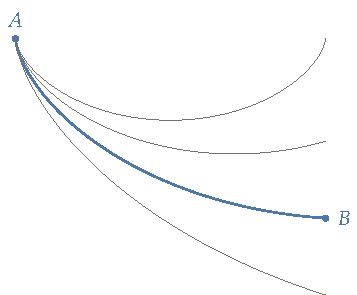
\includegraphics[width=2.5in]{figures/brachistochrone}
	\caption[Short caption to appear in list of figures.]{This is another figure. Some authors have paragraph-like descriptions of their figures that they put into the caption. This is acceptable, but readers don't really want or need a super long caption showing up in their list of figures. The {\ttfamily caption} command provides a nice solution.}
	\label{fig:brach}
\end{figure}

\section{Bibliography}
Another great feature of \LaTeX{} is that it allows you to create a list or database of books, papers, and other documents that you can easily cite in your document. In engineering, it is common to give your bibliography list the title References and we will follow that convention. \LaTeX{} automatically numbers the citations and builds a bibliography for you.\footnote{The building of your bibliography is actually done by {\ttfamily BibTeX}. If you use an IDE to work with \LaTeX, this may not be obvious to you.} The bibliography is typeset according the the style you specify. We recommend the {\em IEEEtran} bibliography style that produces a numbered list in order of citation. For this document, the file {\ttfamily references.bib} contains the bibliographic reference information that's available for citation in the thesis document. Each reference is given a cite key (a label) that is used to cite the reference. For example, here is a reference to a book~\cite{book1} and a reference to a doctoral dissertation~\cite{doctoral1}. Journal articles, such as~\cite{journal1}, are treated differently than conference papers (e.g.,~\cite{conference1}) since their references require slightly different information. For each reference entry in your {\ttfamily .bib} file, different information fields will have to be populated. Examples of these fields include, {\em author}, {\em title}, {\em year}, and so on. Different types of publications will have different required fields for you to fill out. There are other types of citations that you may use, such as book chapters and websites. You can manually edit your {\ttfamily .bib} file with a text editor, or you can use one of the several popular apps that are available for editing and organizing your bibliography information.

\section{Use of Units}
Units should be appropriately used for all measurements and data presented in the document. Standard abbreviations for units (e.g., m for meters, N for newtons, in. for inches) should be used whenever data is presented. For example, the shaft was 1.23 cm in diameter. Notice that there is a space between the number and the unit, and the unit is typeset in vertical (roman) text and is {\em not italicized}. Italics is reserved for emphasis and for mathematical variables. Periods are not used after abbreviations except in the special case of the abbreviation for inches as in. to avoid confusion with the word in. Units are typically spelled out when they are used without data. For example, newtons are a measure of force, while kilograms are a measure of mass.

\section{Capitalization of Reference Labels}
Throughout your document, you will refer to figures, tables, equations, chapters, appendices, and sections by name (e.g., Figure 2.1, Section 3.4, Equation 2.1, and so on). You may choose to capitalize these reference labels, or to leave them uncapitalized (e.g., figure 2.1, section 3.4, equation 2.1). The choice is yours, just be consistent -- all reference labels should be capitalized, or uncapitalized. 

\section{Algorithms}
Software and algorithm development can play an important role in graduate research. Rather than including software code, particularly in the body of the thesis, presenting your algorithms in the form of pseudo-code may be more desirable. The {\ttfamily algorithm} package in \LaTeX{} provides tools for clearly presenting your algorithms. A simple example of the use of this package is presented in Algorithm~\ref{alg:ekf}.

\begin{algorithm}
	\caption{{\color{black} Continuous-discrete extended Kalman filter.}} \label{alg:ekf}
	\begin{algorithmic}[1]
	    \State Initialize:  $\hat{x} = 0$.
	    \State Pick an output sample rate $T_{\textit{out}}$ that is much less than
	    the sample rates of the sensors.
	    \State At each sample time $T_{\textit{out}}$:
	    \For{$i=1$ to $N$}
	        \State $\hat{x} = \hat{x} + \left(\frac{T_{\textit{out}}}{N}\right) \left( f(\hat{x}, u)\right)$
	        \State $A = \frac{\partial{f}}{\partial{x}}$
	        \State $P = P + \left(\frac{T_{\textit{out}}}{N}\right)
	        \left(AP+PA^T + GQG^T\right)$
	    \EndFor
	    \If{a measurement has been received from sensor $i$}
	        \State $C_i = \frac{\partial{c_i}}{\partial{x}}$
	        \State $L_i = PC_i^T(R_i+C_iPC_i^T)^{-1}$
	        \State $P = (I-L_iC_i)P$
	        \State $\hat{x} = \hat{x} +  L_i\left( y_i - c_i( \hat{x})
	        \right)$.
	    \EndIf
	\end{algorithmic}
\end{algorithm}


\section{Landscape Drawings and Tables}
If you have a figure or table that is best presented in landscape format on a full page, the {\ttfamily rotating} package in \LaTeX{} provides a convenient way to do this. Figure~\ref{fig:landscape_dwg} on the following page shows an example a landscape-format drawing.
\begin{sidewaysfigure}
	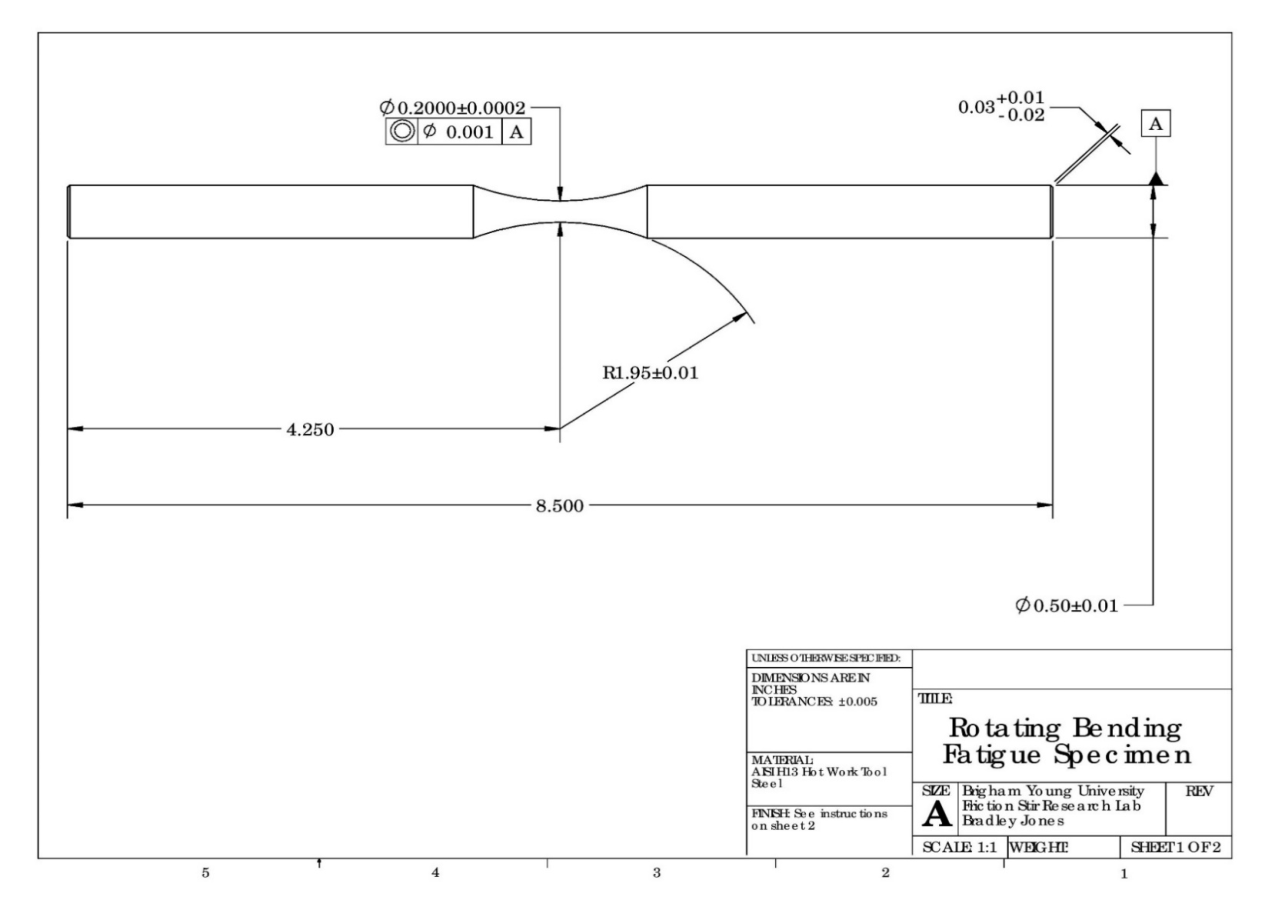
\includegraphics[width=\textwidth]{figures/part_dwg_landscape.pdf}
	\caption{Example of full-page landscape drawing.}
	\label{fig:landscape_dwg}	
\end{sidewaysfigure}


